\chapter{Analisi ammortizzata}
\label{ch:analisi-ammortizzata}
\thispagestyle{chapterInit}

La \textbf{analisi ammortizzata} è una tecnica di analisi degli algoritmi che permette di valutare il tempo richiesto per eseguire, nel caso pessimo, una sequenza di operazioni su una struttura dati. Questa tecnica tiene in considerazione operazioni più o meno costose e se le operazioni costose sono poco frequenti, il costo totale delle operazioni può essere ammortizzato su tutte le operazioni.
\paragraph{Metodi} Gli algoritmi di analisi ammortizzata si basano su tre metodi:
\begin{itemize}
    \item \textbf{Metodo dell'aggregazione} Si calcola la complessita $T(n)$ per eseguire $n$ operazioni in sequenza nel \textbf{caso pessimo}
    \item \textbf{Metodo degli accantonamenti}: Alle operazioni vengono assegnati \textbf{costi ammortizzati} che possono essere maggiori o minori del costo effettivo dell'operazione.
    \item \textbf{Metodo del potenziale}: Lo stato del sistema viene rappresentato da una \textbf{funzione di potenziale}
\end{itemize}
\section{Contatore Binario}
    Sia un contatore binario di $k$ bit con un vettore $A$ di booleani $0/1$ con il bit meno significativo in $A[0]$ e il bit più significativo in $A[k-1]$. Il valore del contatore è dato da: $ x = \sum_{i=0}^{k-1} A[i] \cdot 2^i$. L'operazione $\operatorname{increment}()$ che incrementa il contatore di $1$ è la seguente:
    \begin{algorithm}
        \caption{$\operatorname{increment}(\Int[] A,\Int k)$}
        \begin{algorithmic}
            \State \Int $i \gets 0$
            \While{$i < k \And A[i] = 1$}
                \State $A[i] \gets 0$
                \State $i \gets i+1$
            \EndWhile
            \If{$i < k$}
                \State $A[i] \gets 1$
            \EndIf
        \end{algorithmic}
    \end{algorithm}
    \subsection{Metodo dell'aggregazione}
        Con il metodo dell'aggregazione si calcola la complessità per eseguire $n$ operazioni in sequenza nel caso pessimo (in questo caso avendo una sola operazione non distinguiamo tra caso pessimo e caso medio).\newline
        Si calcola il costo ammortizzato $\frac{T(n)}n$ come \textbf{media} su $n$ operazioni.
        \paragraph{Analisi grossolana} Per $n$ operazioni sono necessari $k=\lceil\log(n+1)\rceil$ bit. Il costo di $\operatorname{increment}()$ è $O(k)$, quindi il costo di $n$ operazioni è $T(n)=O(nk)$ e il costo di una singola operazione è $\frac{T(n)}n=O(k)=O(\log n)$.
        \paragraph{Analisi più stretta} Con la analisi precedente non si tiene conto del fatto che la maggior parte delle operazioni $\operatorname{increment}()$ sono a costo $O(1)$ in quanto non si deve propagare il riporto, inoltre il tempo di esecuzione di una singola operazione è proporzionale al numero di bit che vengono cambiati, ma vengono modificati pochi bit per ogni operazione in quanto non sempre si ha un riporto e non sempre la propagazione del riporto avviene per tutti i bit. Infatti su $8$ bit ad esempio il bit in $A[0]$ viene cambiato ogni operazione, il bit in $A[1]$ viene cambiato ogni $2$ operazioni, il bit in $A[2]$ viene cambiato ogni $4$ operazioni e così via fino al bit in $A[i]$ che viene cambiato ogni $2^i$ operazioni. \newline
        Il costo totale di $n$ operazioni è quindi:
        $$
            T(n)=\sum_{i=0}^{k-1}\left\lfloor\frac{n}{2^i}\right\rfloor\leq n\sum_{i=0}^{k-1}\frac{1}{2^i}\leq n\sum_{i=0}^{\infty}\left(\frac{1}{2}\right)^i=2n
        $$
        Quindi il costo ammortizzato di una singola operazione è $\frac{T(n)}n\leq \frac{2n}n=2=O(1)$.
    \subsection{Metodo degli accantonamenti}
        Si assegna un costo ammortizzato \textit{potenzialmente} distinto ad ogni operazione possibile.\newline
        Il costo ammortizzato può essere diverso dal costo effettivo, le operazioni meno costose vengono caricate di un costo aggiuntivo detto "\textbf{credito}", i crediti accumulati sono usati per pagare le operazioni più costose.
        \paragraph{Obbiettivi} L'obbiettivo è dimostrare che la somma dei costi ammortizzati $a_i$ è un limite superiore ai costi effettivi $c_i$ e che il valore così ottenuto è "poco" costoso. Dunque: $$
            \sum_{i=1}^{n}c_i\leq \sum_{i=1}^{n}a_i
        $$
        Da notare che la dimostrazione deve valere per tutte le sequenze (caso pessimo) e il credito dopo l'operazione $t$-esima è espresso dalla seguente formula: $$
            \sum_{i=1}^{t}a_i-\sum_{i=1}^{t}c_i\geq 0
        $$
        Denotando il costo effettivo dell'operazione $\operatorname{increment}:d$ dove $d$ è il numero di bit che vengono cambiati, il costo ammortizzato è $2$ in quanto $1$ per il cambio di un bit da $0$ a $1$ e $1$ per il cambio di un bit da $1$ a $0$. Allora ne consegue che:\begin{itemize}
            \item In ogni istante, il credito è pari al numero di bit a $1$.
            \item Il costo totale è un $O(n)$.
            \item Il costo ammortizzato di una singola operazione è $O(1)$.
        \end{itemize}
    \subsection{Metodo del potenziale}
        Come anticipato il metodo del potenziale prevede l'utilizzo di una funzione di potenziale $\Phi$ che associa ad uno stato $S$ della struttura data la "quantità di lavoro" $\Phi(S)$ che è stato contabilizzato nell'analisi ammortizzata, ma non ancora eseguito. Con un parallelismo tratto dalla "fisica" $\Phi(S)$ rappresenta la quantità di energia potenziale che è stata accumulata nello stato $S$ e che può essere liberata in futuro.
        \paragraph{Costo Ammortizzato} Il costo ammortizzato di un'operazione $a_i$ è definito come: $$
            a_i=c_i+\Phi(S_i)-\Phi(S_{i-1})
        $$
        dove $c_i$ è il costo reale dell'operazione $a_i$ e $S_i$ è lo stato associato alla $i$-esima operazione. \newline
        Il costo ammortizzato di una sequenza di operazioni è definito come: $$
            \begin{aligned}
                A=&\sum_{i=1}^{n}a_i\\
                =&\sum_{i=1}^{n}\left(c_i+\Phi(S_i)-\Phi(S_{i-1})\right)\\
                =&\underbrace{\sum_{i=1}^{n}c_i}_{C}+\sum_{i=1}^{n}\left(\Phi(S_i)-\Phi(S_{i-1})\right)\\
                =&C+\Phi(S_1)-\Phi(S_0)+\Phi(S_2)-\Phi(S_1)+\ldots+\Phi(S_n)-\Phi(S_{n-1})\\
                =&C+\Phi(S_n)-\Phi(S_0)
            \end{aligned}
        $$
        Se la variazione di potenziale è non negativa, allora il costo ammortizzato $A$ è un limite superiore al costo reale $C$.
        \paragraph{Analisi del Contatore Binario} Scegliamo come funzione potenziale $\Phi$ il numero di bit a $1$ nel contatore binario. Allora nell'operazione $\operatorname{increment}()$ definiamo $t$ come il numero di bit a $1$ incontrati a partire da $A[0]$. Il costo effettivo dell'operazione è $1+t$, la variazione di potenziale è $1-t$ e il costo ammortizzato è $1+t+1-t=2$. In quanto di "media" il costo di un'operazione è $2$ e il costo totale di $n$ operazioni è $2n$ il costo ammortizzato di una singola operazione è $O(1)$.
\section{Vettori Dinamici}
    Il problema della gestione di un vettore dinamico è uno dei problemi più comuni in informatica. 
    \subsection{Inserimento}
        La dimensione di un vettore è fissa e se si vuole aggiungere un elemento in coda al vettore, se il vettore è pieno, bisogna allocare dello spazio aggiuntivo. 
        In un vettore inoltre il costo di un inserimento nella posizione $n$ è $O(n)$ in quanto bisogna spostare tutti gli elementi di una posizione, mentre il costo di un inserimento in coda è $O(1)$ e quindi prediligiamo l'inserimento in coda.
        \paragraph{Soluzione} Si può risolvere il problema allocando alla necessità un vettore di dimensione maggiore (di quanto maggiore?) e copiando gli elementi del vettore originale nel nuovo vettore. E.G. \texttt{java.util.Vector}, \texttt{java.util.ArrayList}.\newline
        Anche se possano sembrare simili uno di questi due metodi è più efficiente dell'altro: \begin{itemize}
            \item \texttt{java.util.Vector} una un incremento fisso della dimensione del vettore, ad esempio di $10$ elementi.
            \item \texttt{java.util.ArrayList} raddoppia la dimensione del vettore.
        \end{itemize}
        Ora è vero che il costo di raddoppio è maggiore rispetto all'incremento fisso, ma in quanto a lungo andare il costo del raddoppio è ammortizzato su $n/2$ operazioni, il costo ammortizzato di un inserimento è $O(1)$. Questo è dimostrabile e esplicabile dalla seguente funzione:
        $$
            c_i=\begin{cases}
                i & \exists k\in\mathbb{Z}_0^+:i=2^k+1\\
                1 & \text{altrimenti}
            \end{cases}
        $$
        Il costo totale dell'inserimento è quindi $T(n)=\sum_{i=1}^{n}c_i=O(n)$ e il costo ammortizzato di un inserimento è $\frac{T(n)}n=\frac{O(\cancel{n}^1)}{\cancel{n}}=O(1)$.
    \subsection[Cancellazione]{Cancellazione - e qui le cose si complicano}
        Prima di analizzare il costo ammortizzato della cancellazione bisogna chiedersi:\begin{itemize}
            \item Quanto costa togliere un elemento da un vettore?
            \item Quanto costa togliere un elemento da un vettore \textbf{non ordinato}?
        \end{itemize}
        Il costo di una cancellazione in un vettore ordinato è $O(n)$ in quanto bisogna spostare tutti gli elementi di una posizione, mentre il costo di una cancellazione in un vettore non ordinato è $O(1)$ in quanto si può spostare l'ultimo elemento al posto dell'elemento da cancellare. \newline
        Detto ciò necessitiamo di ridurre la dimensione del vettore per evitare sprechi di memoria, ma quale è il \textbf{fattore di carico} $\alpha=\frac{\text{dim}}{\text{capacità}}$ che dobbiamo considerare? (Considerando che quando contraiamo il vettore dobbiamo allocare un nuovo vettore, copiare gli elementi e de-allocare il vecchio vettore).
        \paragraph{Strategia Banale}
            Una strategia banale è quella di ridurre la dimensione del vettore quando $\alpha\leq\frac{1}{2}$ il che sembrerebbe una strategia ragionevole, ma in realtà non lo è. Infatti quando consideriamo la cancellazione per la definizione di analisi ammortizzata dobbiamo considerare il caso pessimo nel quale le istruzioni vengono eseguite, finché esiste una sola istruzione che può essere eseguita allora eseguire $n$ operazione ha solo un caso che quindi coincide con il caso pessimo. Se invece consideriamo due istruzioni (inserimento e cancellazione) allora con un fattore di carico $\alpha=\frac{1}{2}$ abbiamo un caso pessimo che si presenta come segue:
            $$\begin{array}{l c c c c c c c c c c c c c}
                \texttt{Ops:} & \texttt{I} & \texttt{I} & \texttt{I} & \texttt{I} & \texttt{I} & \texttt{R} & \texttt{I} & \texttt{R} & \texttt{I} & \texttt{R} & \texttt{I} & \texttt{R} & \texttt{I}\\
                \texttt{Dim:} & 1 & 2 & 3 & 4 & 5 & 4 & 5 & 4 & 5 & 4 & 5 & 4 & 5\\
                \texttt{Cap:} & 8 & 8 & 8 & 8 & 8 & 4 & 8 & 4 & 8 & 4 & 8 & 4 & 8
            \end{array}$$
            Sostanzialmente in questo caso pessimo ad ogni operazione di cancellazione si ha un costo $O(k)$ in quanto bisogna copiare tutti gli elementi nel nuovo vettore.
        \paragraph{Strategia Ottimale}
            La strategia ottimale è quella di ridurre la dimensione del vettore quando $\alpha\leq\frac{1}{4}$, in quanto in questo modo il costo ammortizzato di una cancellazione è $O(1)$. Infatti se consideriamo il caso pessimo in cui ad ogni cancellazione si riduce la dimensione del vettore, il costo totale di $n$ operazioni è $O(n)$ e il costo ammortizzato di una singola operazione è $O(1)$.
        \subsubsection{Funzione di potenziale}
            Possiamo definire una funzione di potenziale $\Phi$ come segue:
            $$
                \Phi = \begin{cases}
                    2\cdot \text{dim} - \text{cap} & \alpha\geq \frac{1}{2}\\
                    \text{cap}/2 - \text{dim} & \alpha\leq \frac{1}{2}
                \end{cases}
            $$
            Quindi il carico dopo una espansione/contrazione sarà $\alpha=\frac12$ con $\Phi=0$\newline
            Prima di una espansione $\alpha=1$ con $\Phi=\text{dim}$\newline
            Prima di una contrazione $\alpha=\frac14$ dunque $\text{capacità}=4\cdot\text{dim}$ con $\Phi=\text{dim}$.
            \newpage
            Di seguito un grafico della funzione di potenziale $\Phi$ insieme al variare della dimensione $size$ e alla capacità $capacity$.
            \begin{figure}[H]
                \centering
                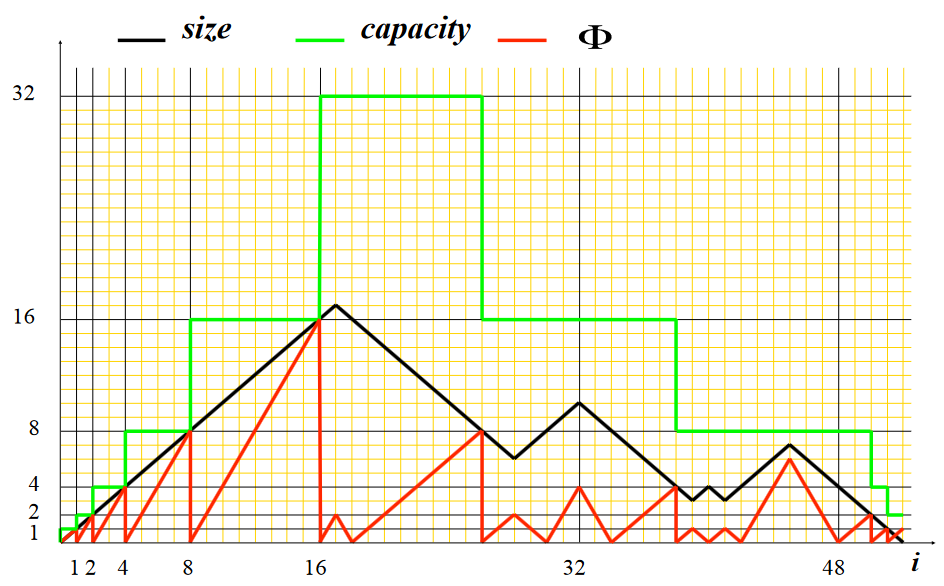
\includegraphics[width=0.5\textwidth]{08/graficoPhiVettore.png}
                \caption{Grafico della funzione di potenziale $\Phi$}
            \end{figure}